\section{Experiments and Results}

\subsection{Dataset}
We used peptide sequences from the Anthem dataset \cite{mei2021anthem}. It consists of 539019, 179673, and 172580 samples for training, validation, and testing, respectively. In more detail, in Fig. S1, we present the distribution of samples by k-mers; 9-mers comprise the majority of samples in the database.

\subsection{Binary classifier and metrics}
The pMHC binding prediction problem is a regression problem. Nonetheless, based on the dataset employed in this study, it could also be approached as a binary classification problem by selecting an appropriate threshold. Moreover, the machine learning metrics used in this work are: Accuracy (Acc.), Precision (Precis.), Recall, F1-score (F1-sc), and Area Under the Curve (AUC).

\subsection{Vanishing gradients}
At the beginning of the experiments, the bigger models suffered from the vanishing gradients problem. Thus, according to best practices to fine-tune the BERT model \cite{mosbach2020stability}, we evaluated lower learning rates, increased the warmup steps in the learning scheduler, and used ADAM with bias correction. So, we evaluated three configurations: (c3) $lr=2e-5$ and 20k warnup steps, (c4) $lr=1e-5$ and 100k warnup steps, and (c5) $lr=2e-6$ and 200k warnup steps. In Fig. \ref{fig:loss}, the loss comparison during training is plotted. In this case, we see that configuration three is good for the smaller model ESM2(t6); however, the same configuration didn't work for the bigger model ESM2(t33). Moreover, in Fig. \ref{fig:t6_c3_gradients} the layer one's gradients of ESM2(t6) show a normal behavior; meanwhile, in Fig. \ref{fig:t33_c3_gradients}, we can see how gradients of the bigger model tend to zero. Thus, configuration four and five were evaluated; sadly, configuration four also went to vanishing gradients. Meanwhile, configuration five overcame that problem according to Fig. \ref{fig:t33_c5_gradients}. For that reason, Configuration Five was applied to the following experiments.

\begin{figure}[h]
	\centering
	
	\begin{subfigure}[b]{0.45\textwidth}
		\centering
		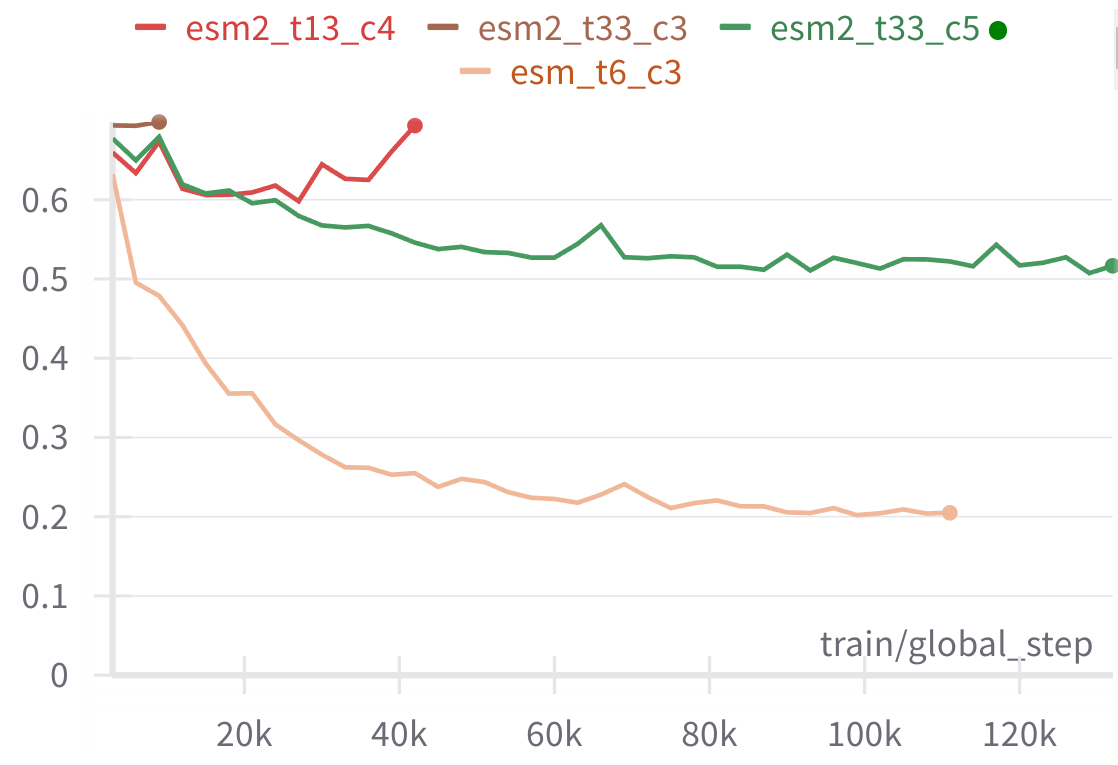
\includegraphics[width=\textwidth]{../img/results/loss2}
		\caption{Loss}
		\label{fig:loss}
	\end{subfigure}
	\hfill
	\begin{subfigure}[b]{0.45\textwidth}
		\centering
		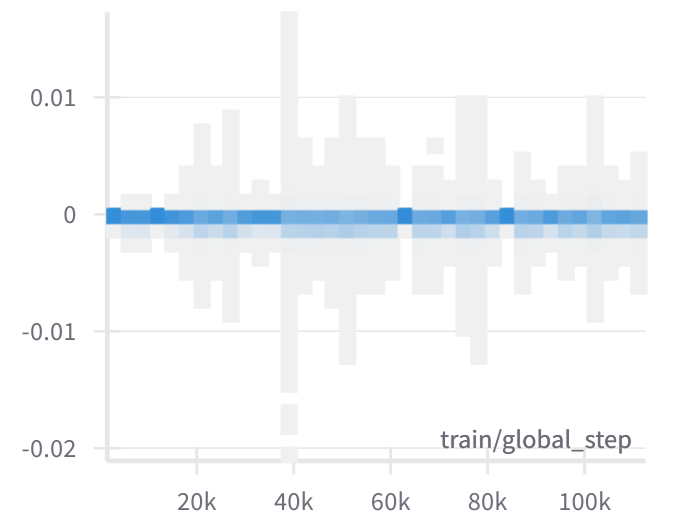
\includegraphics[width=\textwidth]{../img/results/t6_c3_gradients}
		\caption{ESM2(t6) Configuration 3.}
		\label{fig:t6_c3_gradients}
	\end{subfigure}
	\hfill
	\begin{subfigure}[b]{0.45\textwidth}
		\centering
		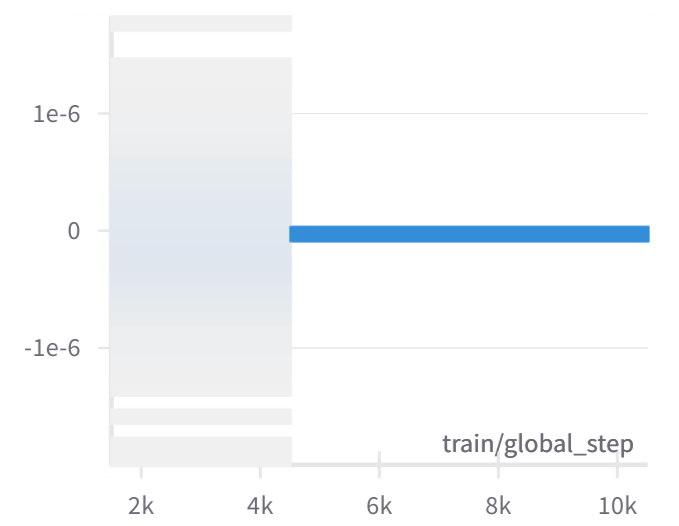
\includegraphics[width=\textwidth]{../img/results/t33_c3_gradients}
		\caption{ESM2(t33) Configuration 3.}
		\label{fig:t33_c3_gradients}
	\end{subfigure}
	\hfill
	\begin{subfigure}[b]{0.45\textwidth}
		\centering
		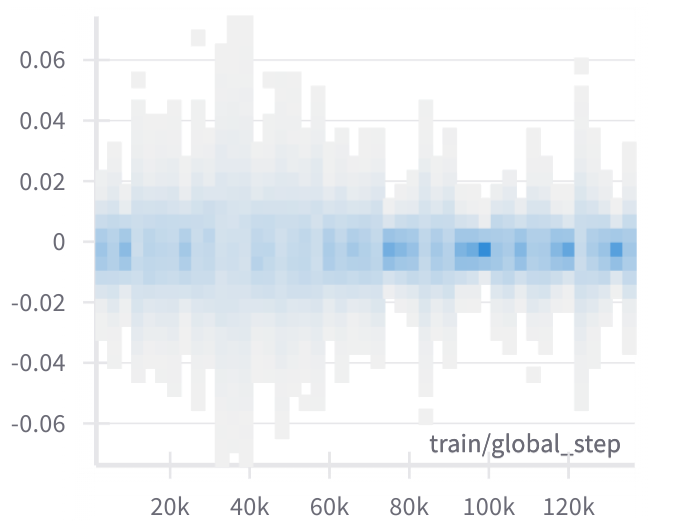
\includegraphics[width=\textwidth]{../img/results/t33_c5_gradients}
		\caption{ESM2(t33) Configuration 5.}
		\label{fig:t33_c5_gradients}
	\end{subfigure}
	
	%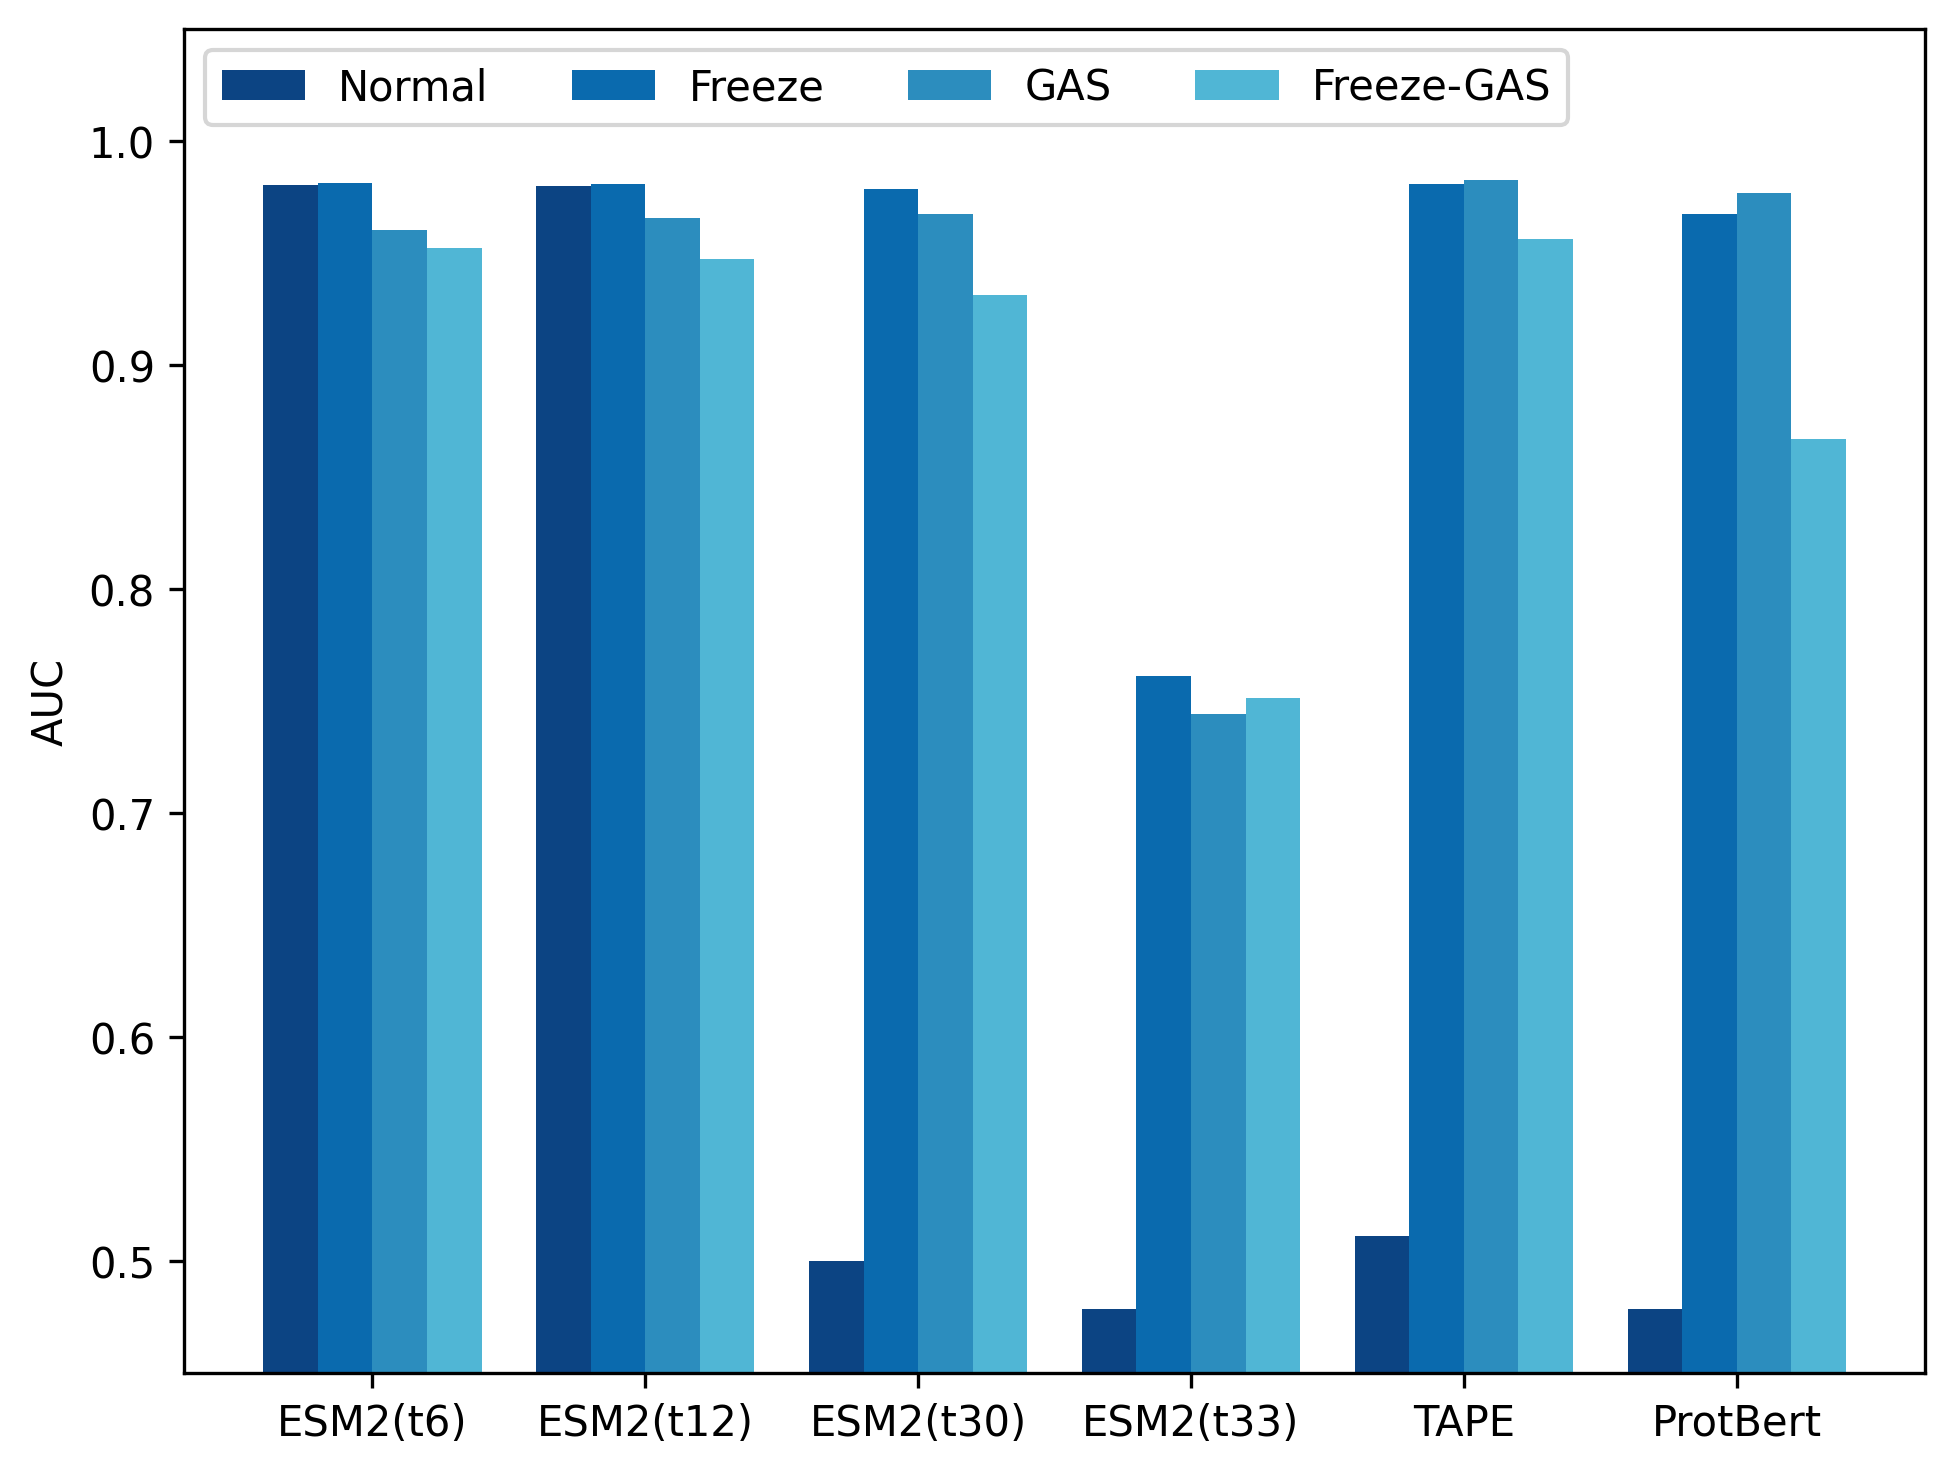
\includegraphics[width=0.42\textwidth]{../img/results/metrics_comparion_by_model}	
	
	\caption{(a) Loss during training of three configurations varying the learning rate and warmup steps. (b) First layer's gradients of ESM2(t6) using third configuration. (c) First layer's gradients of ESM2(t33) using the fourth configuration. (d) First layer's gradients of ESM2(t33) using the fifth configuration.}
	\label{fig:training}
\end{figure}


\subsection{The layer freezing methodology and GAS}

For the layer freezing methodology, we froze all the Transformer's parameters and just trained the BiLSTM block. Using this method speeds up the training and still achieves good performance, as discussed in prior works \cite{merchant2020happens,lee2019would,kovaleva2019revealing}. The performance comparison is presented in Table \ref{tab:comparison_3_epochs}; the suffix 'GAS' signifies the integration of Gradient Accumulation Steps (GAS), while the suffix 'Freeze' is indicative of our application of the layer freezing methodology to the models.

\begin{figure}[h]
	\centering
	
	
	
	\begin{subfigure}[b]{0.45\textwidth}
		\centering
		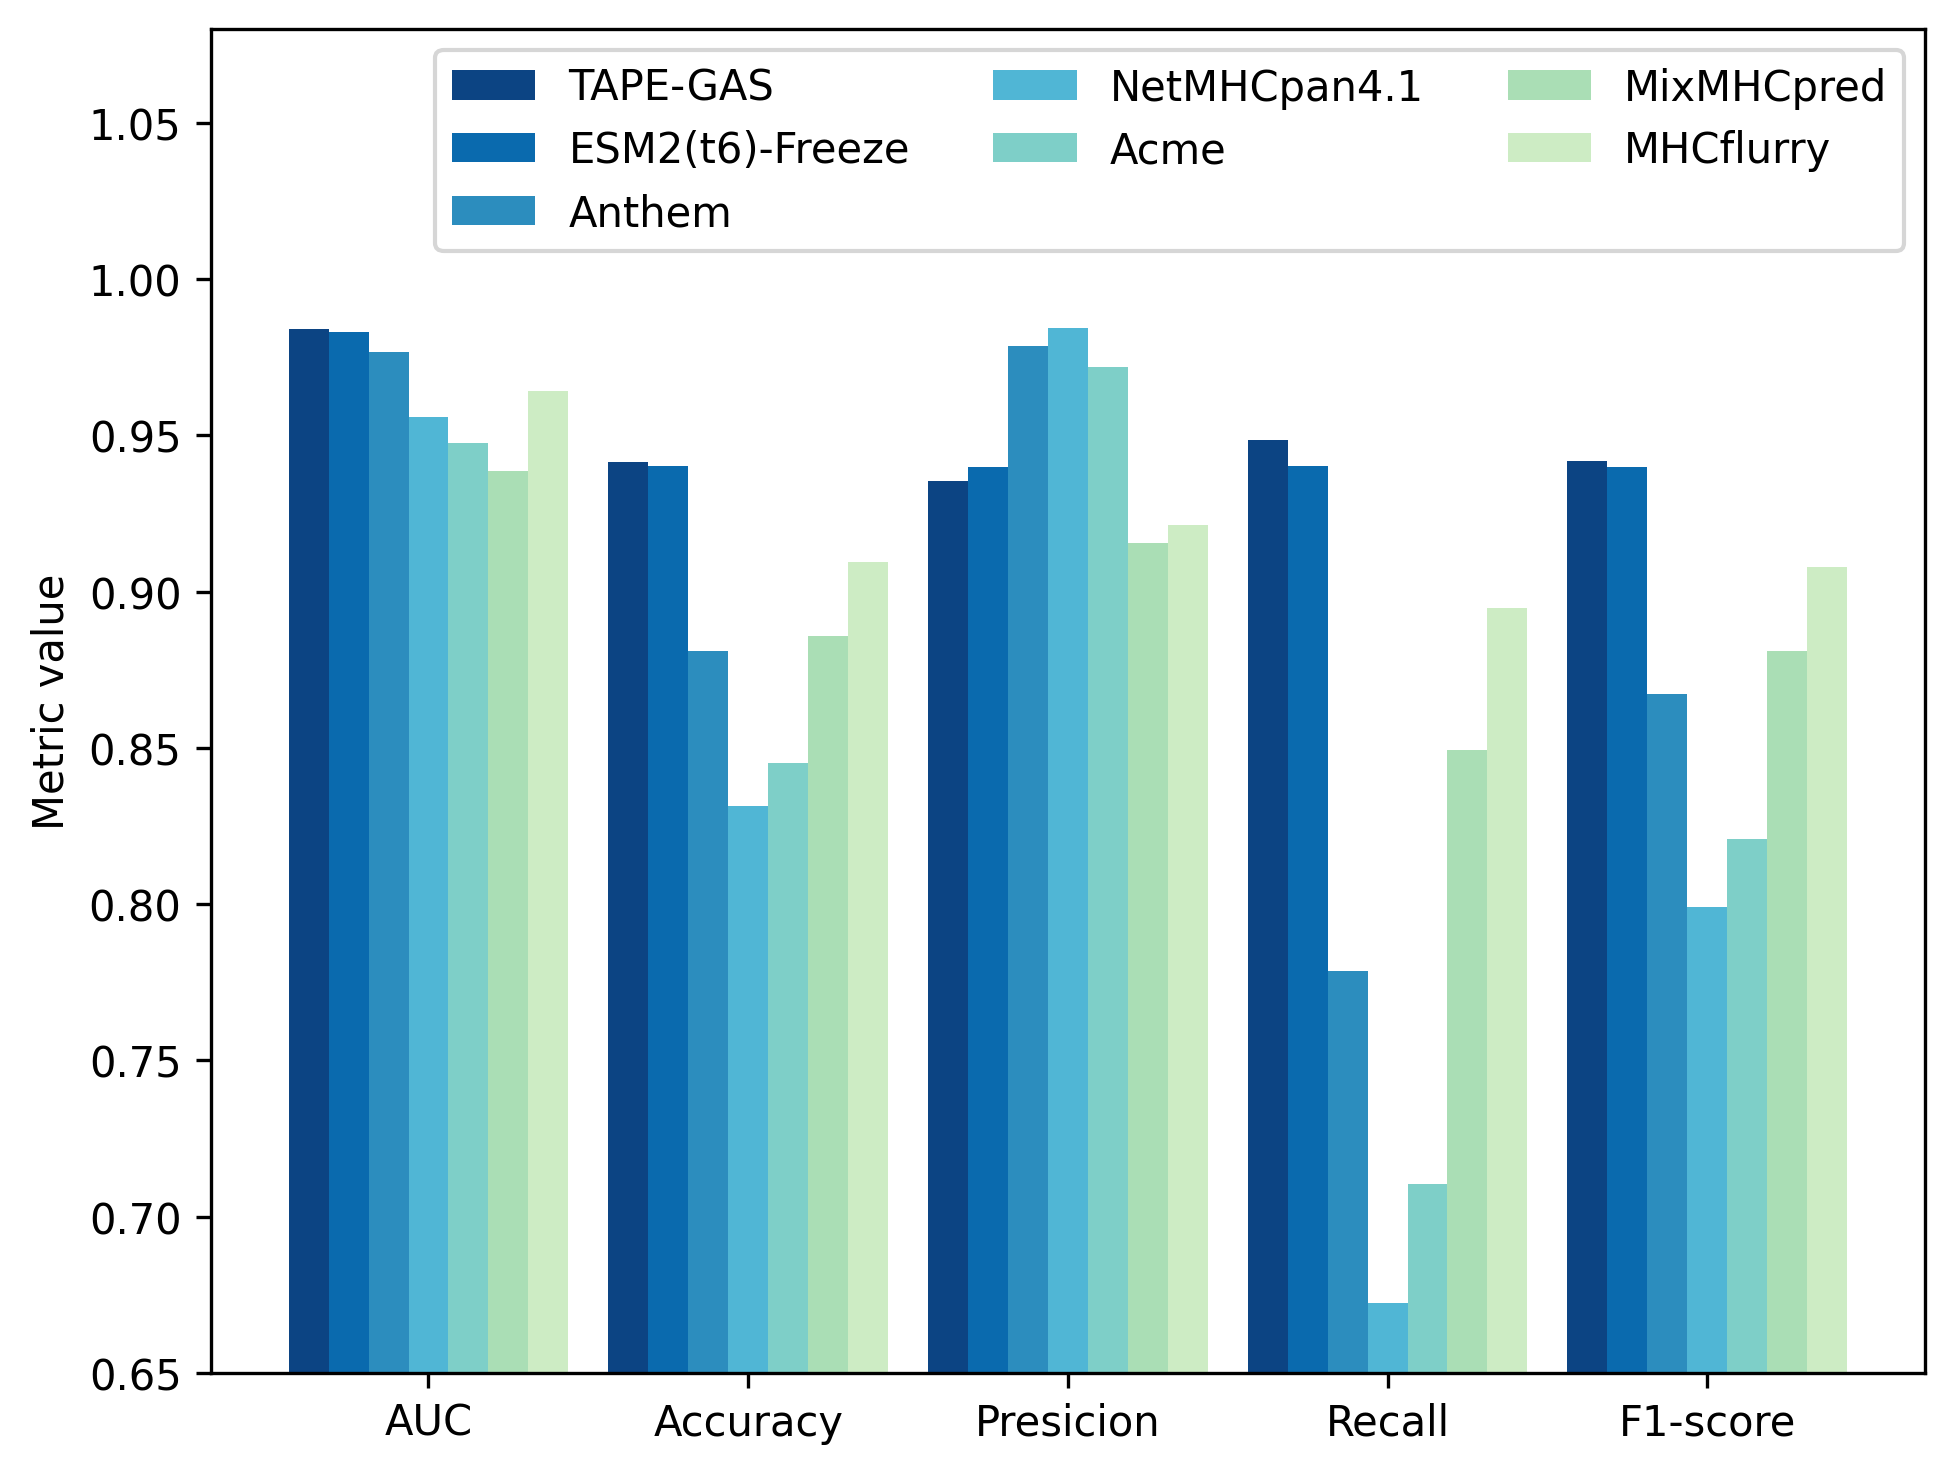
\includegraphics[width=\textwidth]{../img/results/metrics_comparison}
		\caption{Thirty epochs}
		\label{fig:comparison_final}
	\end{subfigure}
	\hfill
	\begin{subfigure}[b]{0.45\textwidth}
		\centering
		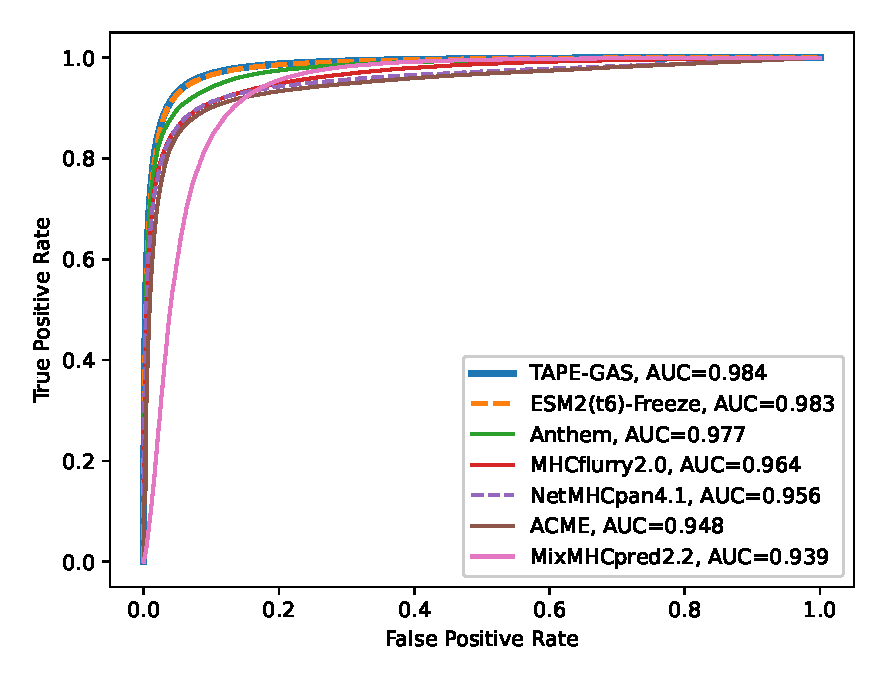
\includegraphics[width=\textwidth]{../img/results/ROC_comparison}
		\caption{ROC curves}
		\label{fig:ROC_comparison_final}
	\end{subfigure}
	
	%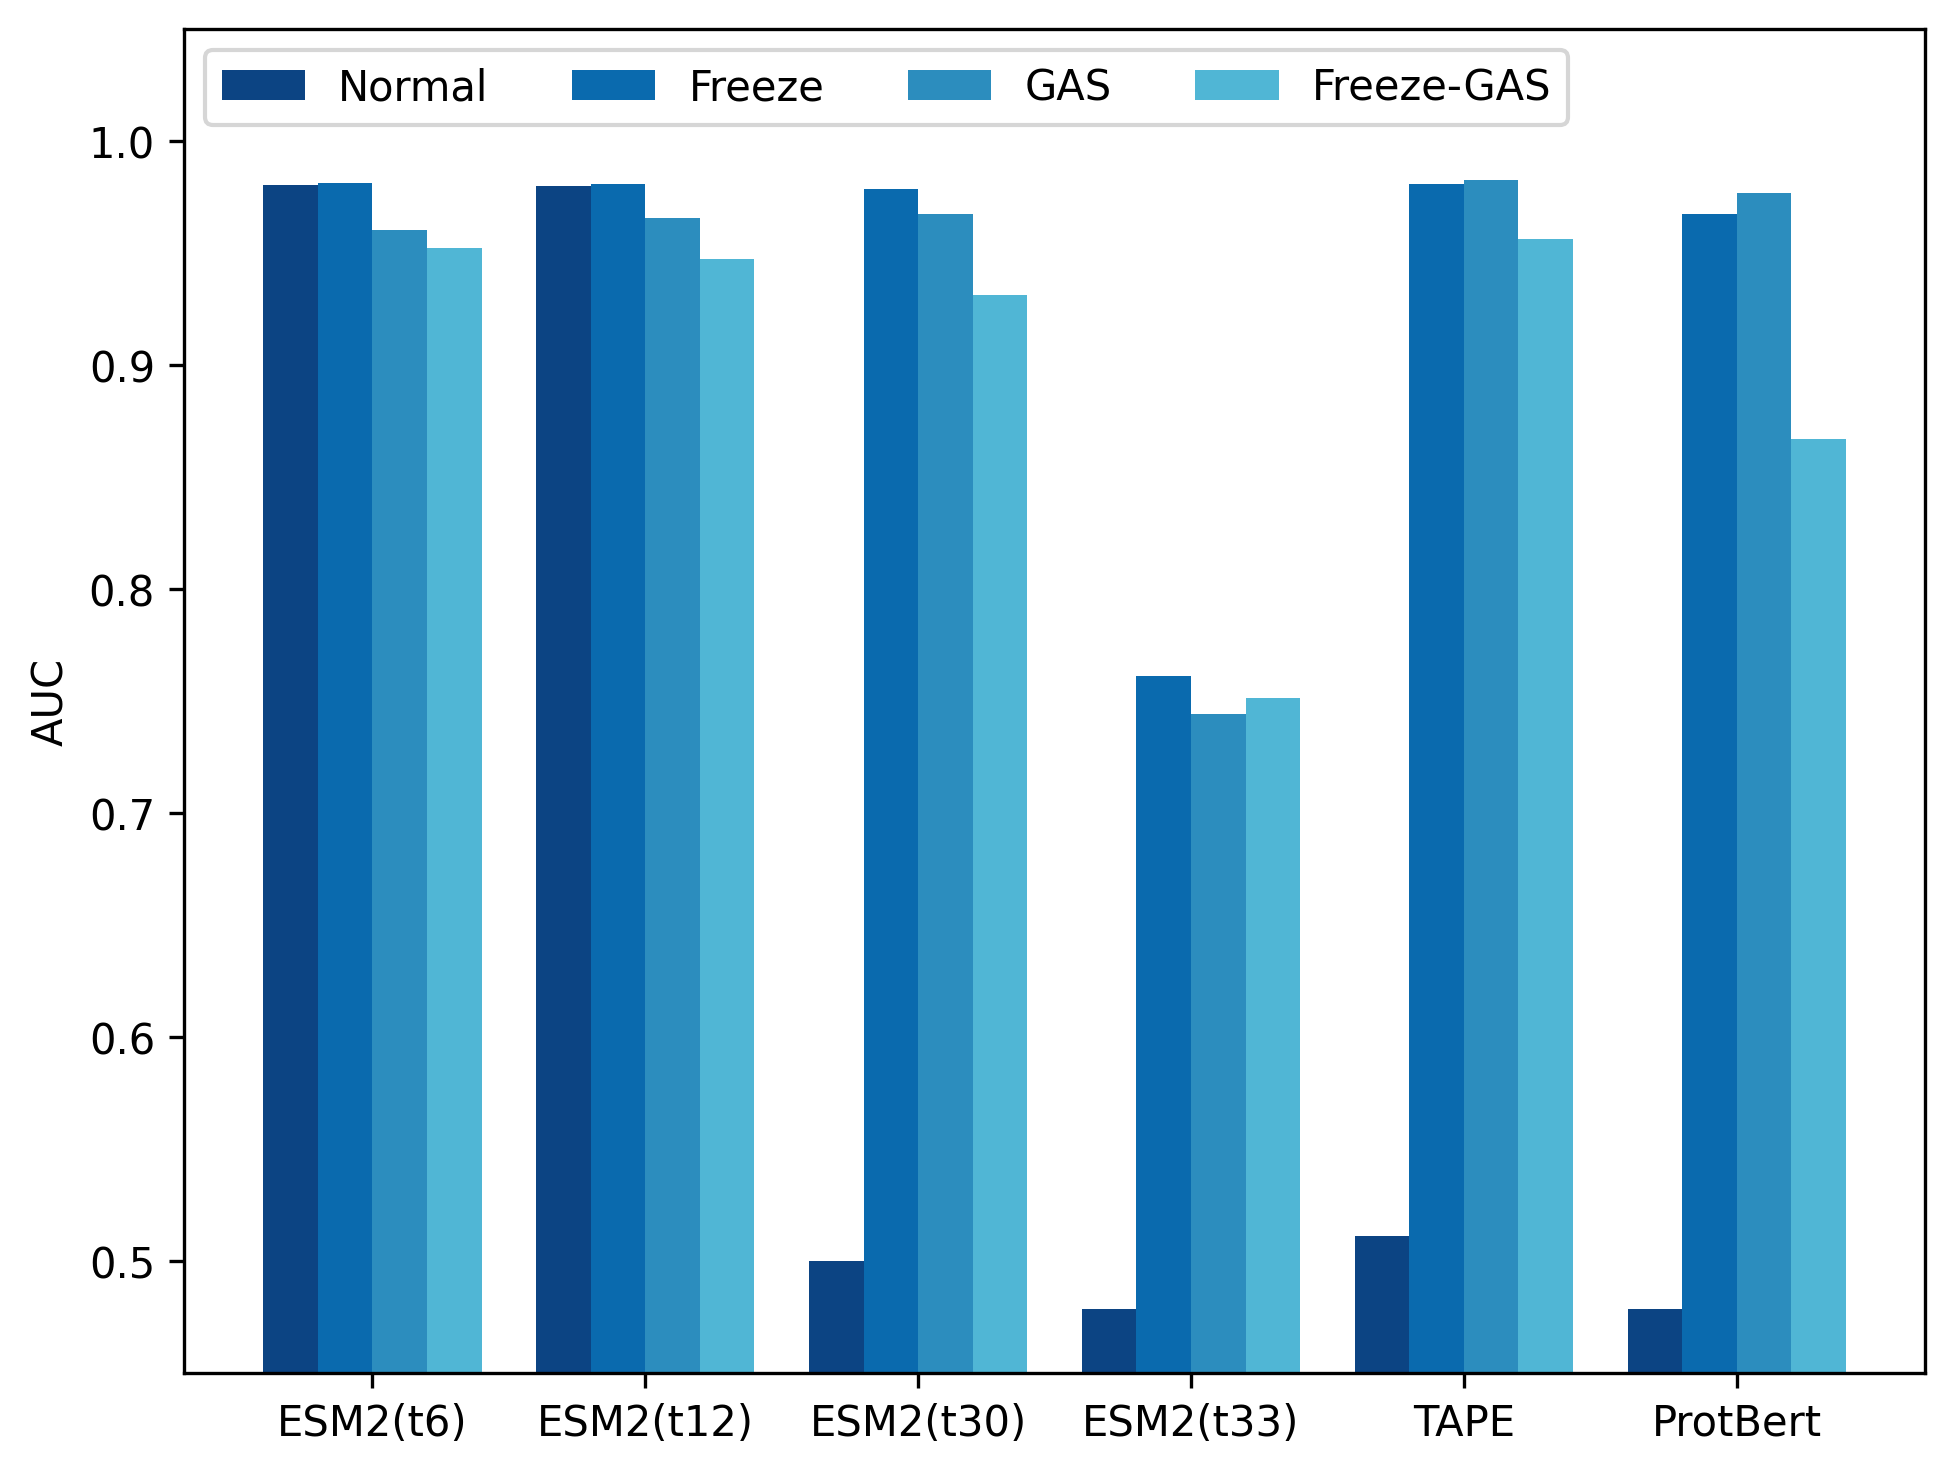
\includegraphics[width=0.42\textwidth]{../img/results/metrics_comparion_by_model}	
	
	\caption{(a) The AUC values for TAPE-GAS and ESM2(t6) trained for 30 epochs, in comparison to state-of-the-art methods. (b) ROC curves for TAPE-GAS and ESM2(t6) trained for 30 epochs, in comparison to state-of-the-art methods.}
	\label{fig:comparison}
\end{figure}





\begin{table}[h]
	\centering
	\caption{Performance evaluation of Transformer models with Gradient Accumulation Steps (GAS) and the layer freezing methodology trained for three epochs. Moreover, the suffix 'Normal' stands for classic training. The inclusion of the suffix 'GAS' in each model signifies the integration of Gradient Accumulation Steps, while the suffix 'Freeze' is indicative of our application of the layer freezing methodology to the models.}
	\label{tab:comparison_3_epochs}
	
	\scriptsize
	\begin{tabular}{llllll} \hline
		\textbf{Model}       & \textbf{Acc.} & \textbf{Precis.} & \textbf{Recall} & \textbf{F1-sc.} & \textbf{AUC}   % & \textbf{MCC}    
		\\ \hline
		ESM2(t6)-Normal             & 0.9344            & \textbf{0.9334}    & 0.9354          & 0.9344            & 0.9805          %& 0.8689          
		\\
		ESM2(t6)-Freeze      & \textbf{0.9351}   & 0.9253             & \textbf{0.9464} & \textbf{0.9357}   & \textbf{0.9812} %& \textbf{0.8704} 
		\\
		ESM2(t6)-GAS         & 0.8986            & 0.8966             & 0.9007          & 0.8986            & 0.9602          %& 0.7973          
		\\
		ESM2(t6)-Freeze-GAS  & 0.8869            & 0.8913             & 0.8806          & 0.8860            & 0.9520          %& 0.7738          
		\\ \hline
		
		
		ESM2(t12)-Normal            & 0.9327            & 0.9243             & 0.9422          & 0.9332            & 0.9799          %& 0.8655          
		\\
		ESM2(t12)-Freeze     & \textbf{0.9344}   & \textbf{0.9251}    & \textbf{0.9451} & \textbf{0.9350}   & \textbf{0.9808} %& \textbf{0.8690} 
		\\
		ESM2(t12)-GAS        & 0.9010            & 0.9279             & 0.8692          & 0.8976            & 0.9655          %& 0.8037          
		\\
		ESM2(t12)-Freeze-GAS & 0.8805            & 0.8556             & 0.9149          & 0.8843            & 0.9475          %& 0.7629          
		\\ \hline
		
		
		ESM2(t30)-Normal             & 0.8923                 & 0.8956                  & 0.9076               & 0.9034                 & 0.9467               %&                & -               %& -               
		\\
		ESM2(t30)-Freeze     & \textbf{0.9303}   & \textbf{0.9185}    & \textbf{0.9440} & \textbf{0.9311}   & \textbf{0.9786} %& \textbf{0.8609} 
		\\
		ESM2(t30)-GAS        & 0.9090            & 0.9167             & 0.8993          & 0.9079            & 0.9675          %& 0.8181          
		\\
		ESM2(t30)-Freeze-GAS & 0.8565            & 0.8156             & 0.9206          & 0.8649            & 0.9312          %& 0.7191          
		\\ \hline
		
		
		ESM2(t33)-Normal            & 0.6797                 & 0.7122                  & 0.8076               & 0.7220                 & 0.7458               %& -               
		\\
		ESM2(t33)-Freeze     & \textbf{0.6818}   & \textbf{0.7139}    & 0.6044          & 0.6546            & \textbf{0.7613} %& 0.3677          
		\\
		ESM2(t33)-GAS        & 0.6767            & 0.6312             & 0.8467          & 0.7233            & 0.7442         % & \textbf{0.3763} 
		\\
		ESM2(t33)-Freeze-GAS & 0.6738            & 0.6254             & \textbf{0.8633} & \textbf{0.7254}   & 0.7514          %& 0.3763          
		\\ \hline
		
		
		TAPE-Normal             & 0.8986                 & 0.8245                  & 0.9045               & 0.8845                 & 0.9267                           
		\\
		TAPE-Freeze          & 0.9342            & 0.9276             & 0.9415          & 0.9345            & 0.9809          %& 0.8684          
		\\
		TAPE-GAS             & \textbf{0.9371}   & \textbf{0.9290}    & \textbf{0.9463} & \textbf{0.9376}   & \textbf{0.9826} %& \textbf{0.8744} 
		\\
		TAPE-Freeze-GAS      & 0.8914            & 0.8851             & 0.8989          & 0.8920            & 0.9564          %& 0.7828          
		\\ \hline
		
		
		ProtBert-Normal          & 0.7456                 & 0.7045                  & 0.7205               & 0.7599                 & 0.7178               %&
		\\
		ProtBert-Freeze      & 0.9083            & 0.9176             & 0.8968          & 0.9071            & 0.9673          %& 0.8168          
		\\
		ProtBert-GAS         & \textbf{0.9138}   & \textbf{0.9569}    & 0.8662          & \textbf{0.9093}   & \textbf{0.9767} %& \textbf{0.8313} 
		\\
		ProtBert-Freeze-GAS  & 0.7864            & 0.7333             & \textbf{0.8988} & 0.8076            & 0.8669          %& 0.5881         
		\\ \hline
	\end{tabular}
\end{table}



For a more detailed comparison, we extended the training epochs of the best-performing models from Table \ref{tab:comparison_3_epochs}, including ESM2(T6) and TAPE, to 30 epochs with early stopping. It is worth noting that ProtBert-BFD was excluded from the analysis due to its poor performance. As indicated in Table \ref{tab:comparison}, the ESM2 models yield their best results when the layer freezing methodology is applied. In contrast, for TAPE, the best results are achieved when using GAS without freezing. Notably, TAPE-GAS and ESM2(t6)-Freeze produced the most favorable outcomes, with TAPE-GAS slightly outperforming ESM2(t6)-Freeze in this regard.




\begin{table}[h]
	\centering
	\caption{Performance evaluation of Transformer models with GAS and the layer freezing methodology, trained for thirty (30) epochs. Moreover, the suffix 'Normal' stands for classic training. The inclusion of the suffix 'GAS' in each model signifies the integration of GAS, while the suffix 'Freeze' is indicative of our application of the layer freezing methodology to the models.}
	\label{tab:comparison}
	\scriptsize
	\begin{tabular}{llllll} \hline
		\textbf{}            & \textbf{Acc.} & \textbf{Precis.} & \textbf{Recall} & \textbf{F1-sc.} & \textbf{AUC}      \\ \hline
		ESM2(t6)-Normal             & 0.9390            & 0.9333             & \textbf{0.9453} & 0.9392            & 0.9797                    \\
		
		ESM2(t6)-Freeze      & \textbf{0.9401}   & \textbf{0.9398}    & 0.9402          & \textbf{0.9400}   & \textbf{0.9830}          \\
		ESM2(t6)-GAS         & 0.9366            & 0.9322             & 0.9413          & 0.9368            & 0.9818                           \\
		ESM2(t6)-Freeze-GAS  & 0.9354            & 0.9326             & 0.9383          & 0.9355            & 0.9813                             \\ \hline
		
		TAPE-Normal        & 0.9086                 & 0.9399                  & 0.9281               & 0.9145                 & 0.9648                                 \\
		TAPE-Freeze          & 0.9395            & \textbf{0.9404}    & 0.9382          & 0.9393            & 0.9815                           \\
		TAPE-GAS             & \textbf{0.9415}   & 0.9352             & \textbf{0.9484} & \textbf{0.9418}   & \textbf{0.9841}            \\
		TAPE-Freeze-GAS      & 0.9359            & 0.9297             & 0.9428          & 0.9362            & 0.9820                    \\ \hline    
	\end{tabular}
\end{table}


\subsection{Comparison with state-of-art methods}
Additionally, we compare the best models: ESM2(t6)-Freeze and TAPE-GAS trained for 30 epochs (see Table \ref{tab:comparison}) with state-of-art methods. We covered NetMHCpan4.1 \cite{reynisson2020netmhcpan}, and MHCFlurry2.0 \cite{o2020mhcflurry} because are well-know baselines methods; and three latest tools such as Anthem \cite{mei2021anthem},  Acme \cite{hu2019acme} and MixMHCpred2.2  \cite{gfeller2023improved}. 
During our evaluation of these tools on the test dataset, we encountered specific considerations for ACME. To ensure a fair assessment, we excluded the following alleles from the evaluation for ACME: HLA-C01:02, HLA-C02:02, HLA-C03:03, HLA-C03:04, HLA-C04:01, HLA-C05:01, HLA-C06:02, HLA-C07:01, HLA-C07:02, HLA-C07:04, HLA-C08:02, HLA-C12:03, HLA-C14:02, HLA-C15:02, HLA-C16:01, HLA-C17:01, HLA-A02:50, HLA-A24:06, HLA-A24:13, HLA-A32:15, HLA-B45:06, and HLA-B83:01. This exclusion was necessary as ACME was unable to predict peptide-MHC binding for these particular alleles,

It's worth noting that the choice of threshold for predicting pMHC binding can vary depending on the specific tool and k-mer used. This variability makes the AUC an ideal metric for comparing methods, as it provides a robust evaluation that isn't sensitive to threshold differences. For that reason, in  Figure \ref{fig:comparison_final} and \ref{fig:ROC_comparison_final}, we present the AUC and ROC curve respectively of TAPE-GAS, ESM2(t6)-Freeze, NetMHCpan4.1, and MHCFlurry2.0, Anthem,  Acme, and MixMHCpred2.2. According to these plots, TAPE-GAS, ESM2(t6)-Freeze got the highest AUC value.

Furthermore, when assessing binary classification performance metrics, we standardized the threshold for TAPE-GAS and ESM2(t6) at 0.5. We maintained a threshold of 0.5 for NetMHCpan4.1, in accordance with its recommended setting, while for ACME, we adhered to a threshold of 0.42, as advised in its documentation. In the case of Anthem, the tool provided binary binding predictions directly. However, for MixMHCpred2.2 and MHCfurry, we determined the optimal threshold values from the test dataset, resulting in 2.7308 and 0.09439, respectively. In Table \ref{tab:final_comparison}, we present a comprehensive comparison between TAPE-GAS and ESM2(t6)-Freeze (trained for 30 epochs), and state-of-the-art methods. The results clearly demonstrate that TAPE-GAS and ESM2(t6)-Freeze consistently outperform the existing state-of-the-art tools across all these metrics: AUC, Accuracy, Recall, F1-score, and MCC. 


\begin{table}[h]
	\centering
	\caption{Performance evaluation of Transformer models TAPE-GAS and ESM2(t6)-Freeze, trained for 30 epochs, against Anthem, NetMHCpan4.1, ACME, MixMHCpred2.2, and MhcFlurry2.0.}
	\label{tab:final_comparison}
	\scriptsize
	\begin{tabular}{lllllll} \hline
		& \textbf{Acc.} & \textbf{Precis.} & \textbf{Recall} & \textbf{F1-sc} & \textbf{AUC}    & \textbf{MCC}    \\ \hline
		TAPE-GAS        & \textbf{0.9415}   & 0.9352             & \textbf{0.9484} & \textbf{0.9418}   & \textbf{0.9841} & \textbf{0.8831} \\
		ESM2(t6)-Freeze & \textbf{0.9401}   & 0.9398             & \textbf{0.9402} & \textbf{0.9400}   & \textbf{0.9830} & \textbf{0.8802} \\
		
		Anthem          & 0.8811            & \textbf{0.9786}    & 0.7787          & 0.8673            & 0.9768          & 0.7785          \\
		NetMHCpan4.1    & 0.8312            & \textbf{0.9844}    & 0.6724          & 0.7991            & 0.9557          & 0.6982          \\
		
		ACME            & 0.8452            & 0.9717             & 0.7105          & 0.8208            & 0.9476          & 0.7165          \\
		MixMHCpred2.2   & 0.8857            & 0.9155             & 0.8493          & 0.8811            & 0.9386          & 0.7733          \\
		MhcFlurry2.0    & 0.9093            & 0.9211             & 0.8948          & 0.9078            & 0.9642          & 0.8189 \\ \hline        
	\end{tabular}
\end{table}


Finally, we show the AUC distribution for TAPE-GAS and ESM2(t6)-Freeze, both trained for 30 epochs, along with Anthem, NetMHCpan4.1, ACME, MixMHCpred2.2, and MHCflurry2.0. In this case, we evaluated each distribution by k-mer (Fig. \ref{fig:auc_distribution}). In all k-mer, TAPE-GAS and ESM2(t6)-Freeze present the highest score. Furthermore, it's worth noting that the compact ESM2(t6)-Freeze model delivers superior results for longer peptides with lengths of 11, 12, 13, and 14.


\begin{figure*}[h]
	\centering
	%\begin{subfigure}[b]{0.3\textwidth}
	%	\centering
	%	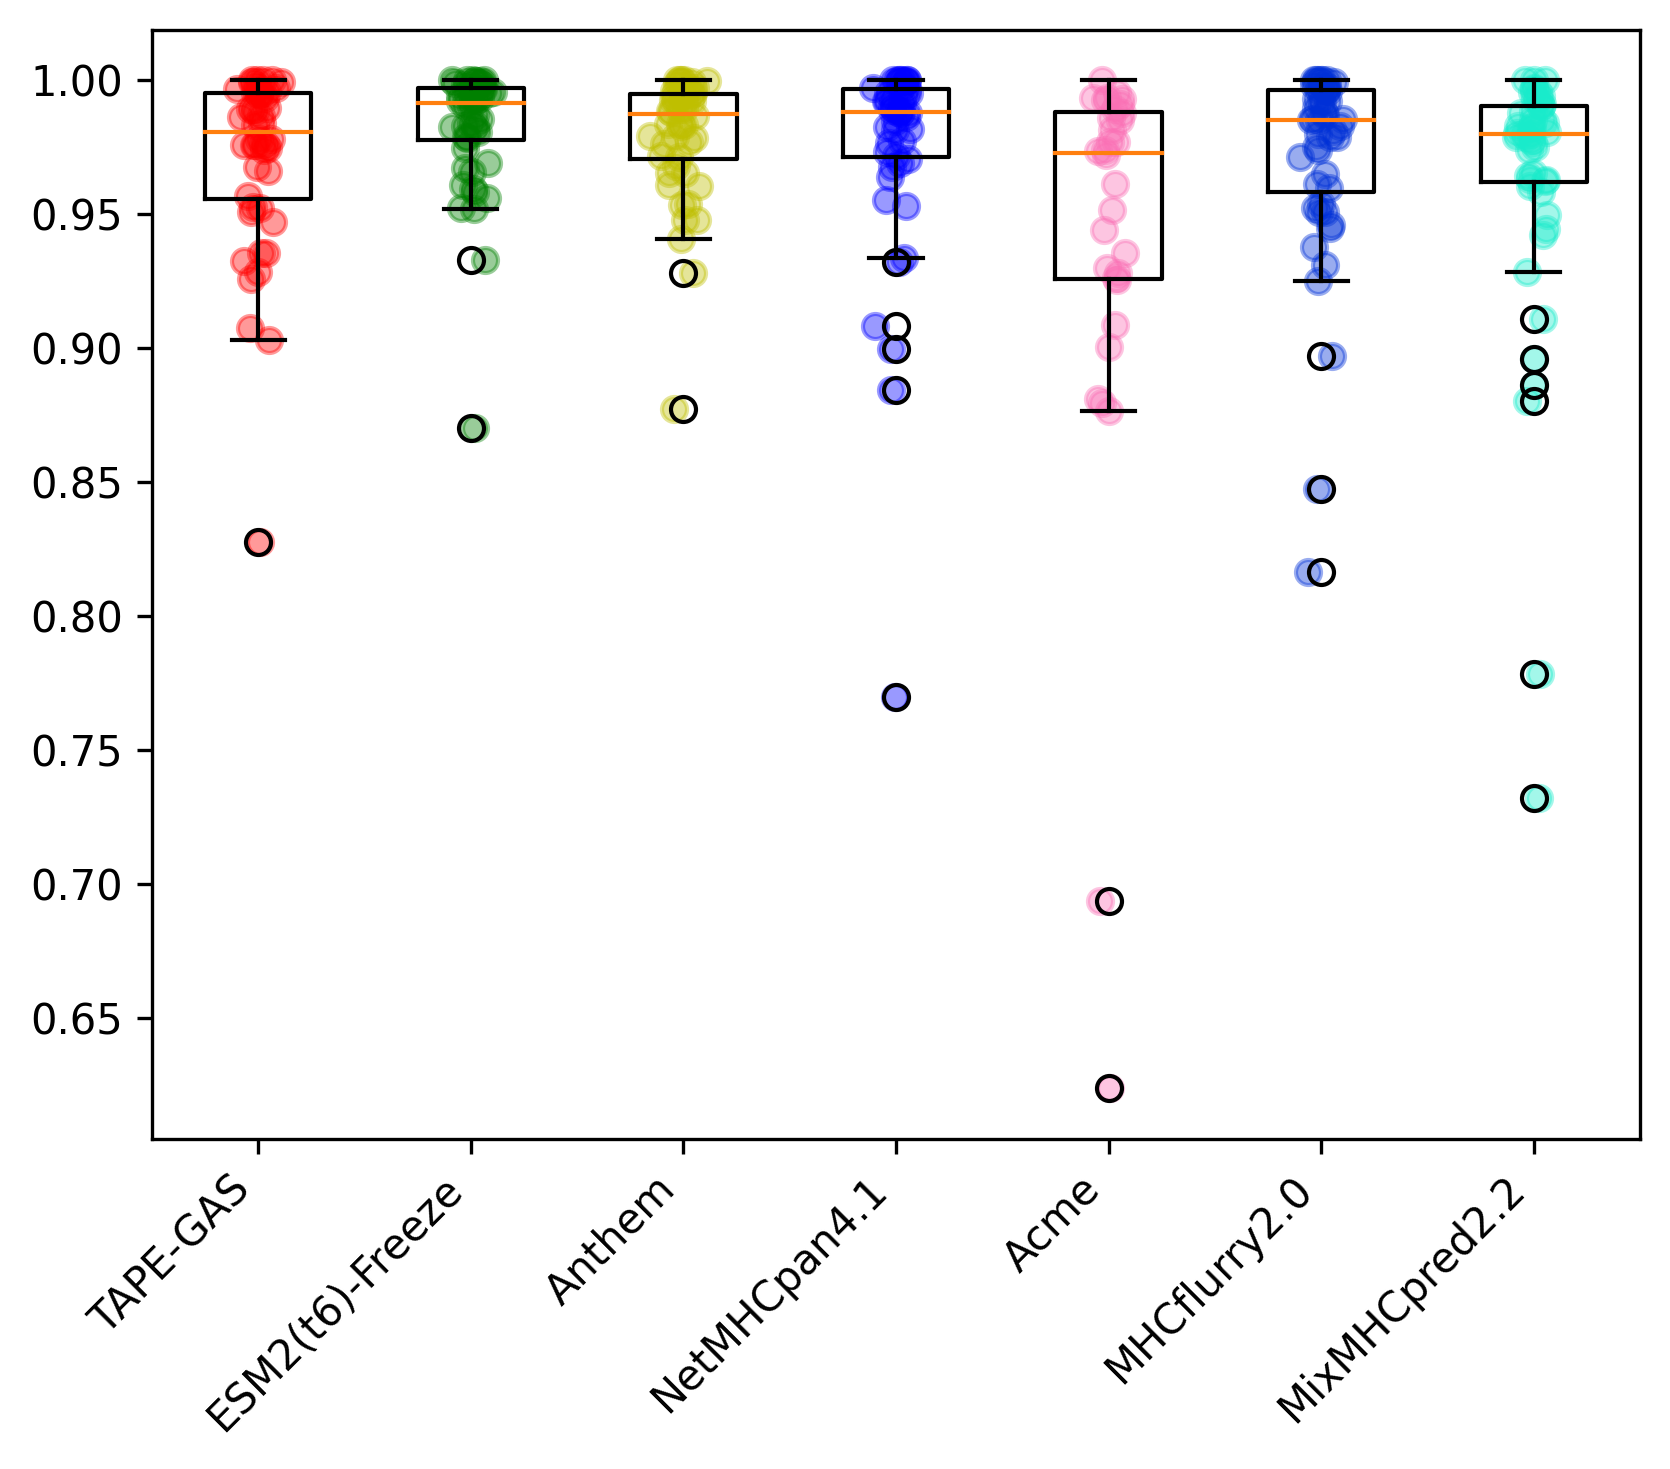
\includegraphics[width=\textwidth]{img/results/auc_distribution_8-mer.eps}
	%	\caption{8-mer}
	%	\label{fig:comparison_8}
	%\end{subfigure}
	%\hfill
	\begin{subfigure}[b]{0.3\textwidth}
		\centering
		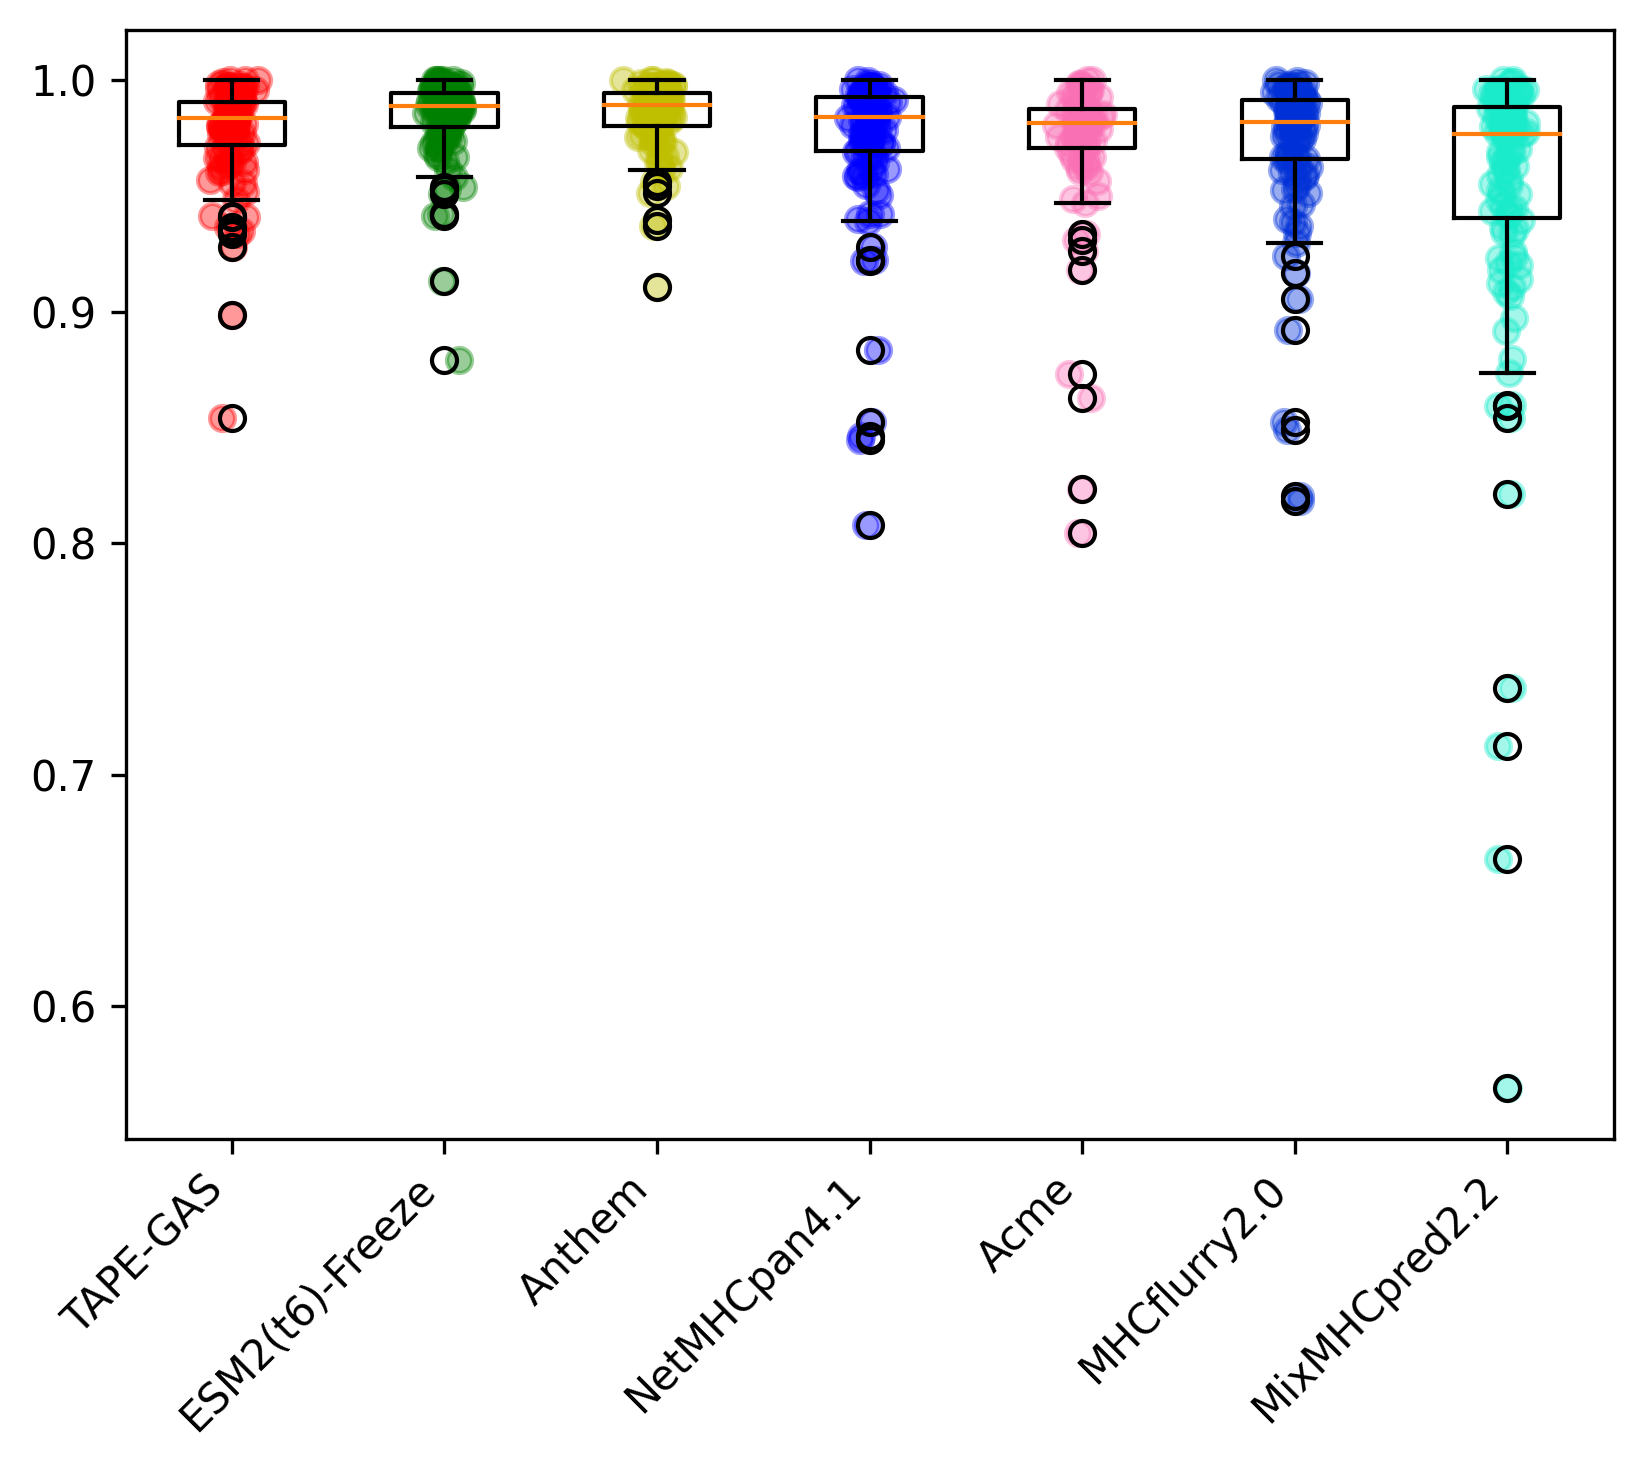
\includegraphics[width=\textwidth]{../img/results/auc_distribution_9-mer}
		\caption{9-mer}
		\label{fig:comparison_9}
	\end{subfigure}
	\hfill
	\begin{subfigure}[b]{0.3\textwidth}
		\centering
		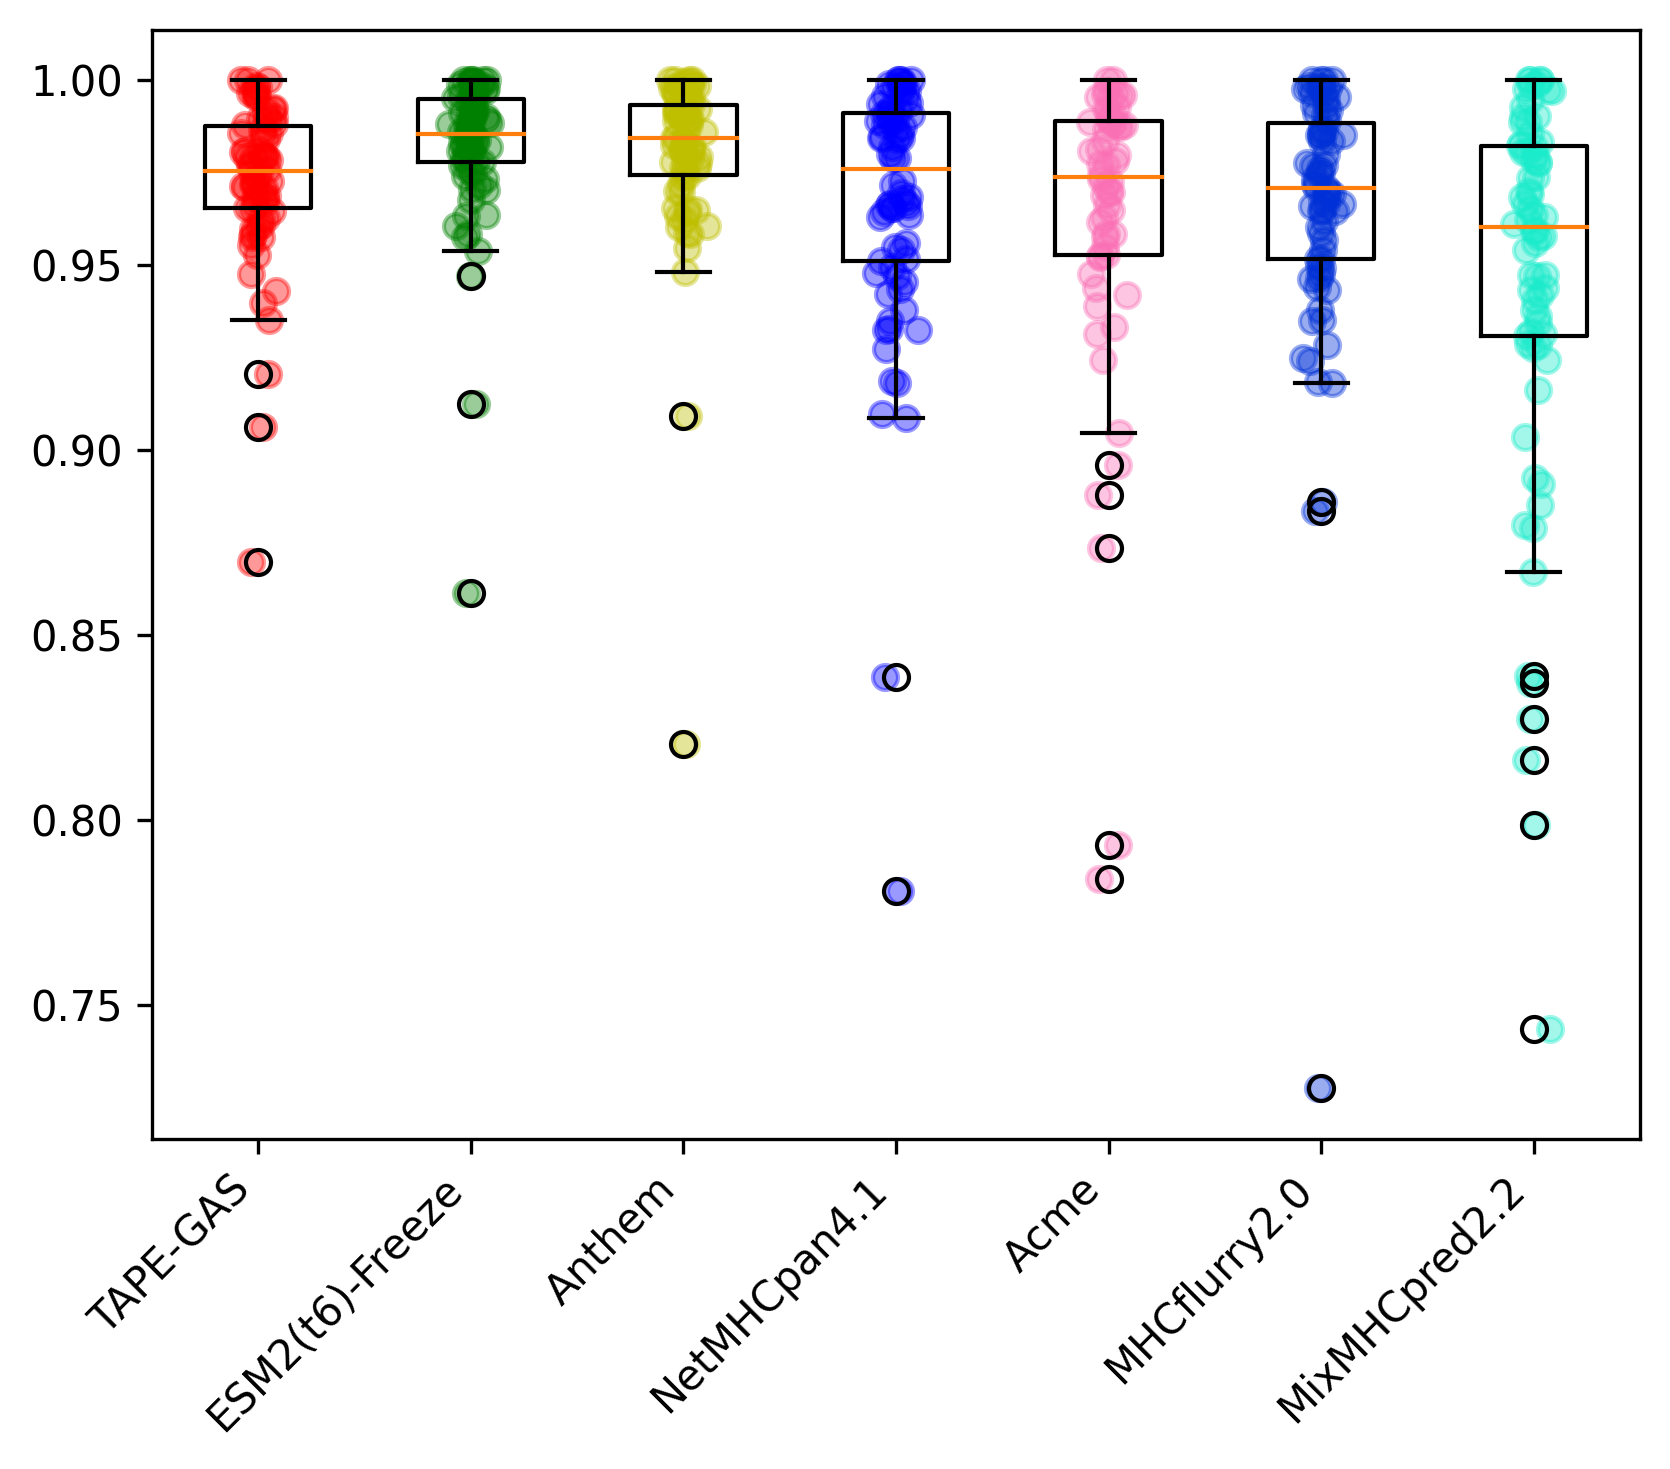
\includegraphics[width=\textwidth]{../img/results/auc_distribution_10-mer}
		\caption{10-mer}
		\label{fig:comparison_10}
	\end{subfigure}
	\hfill
	\begin{subfigure}[b]{0.3\textwidth}
		\centering
		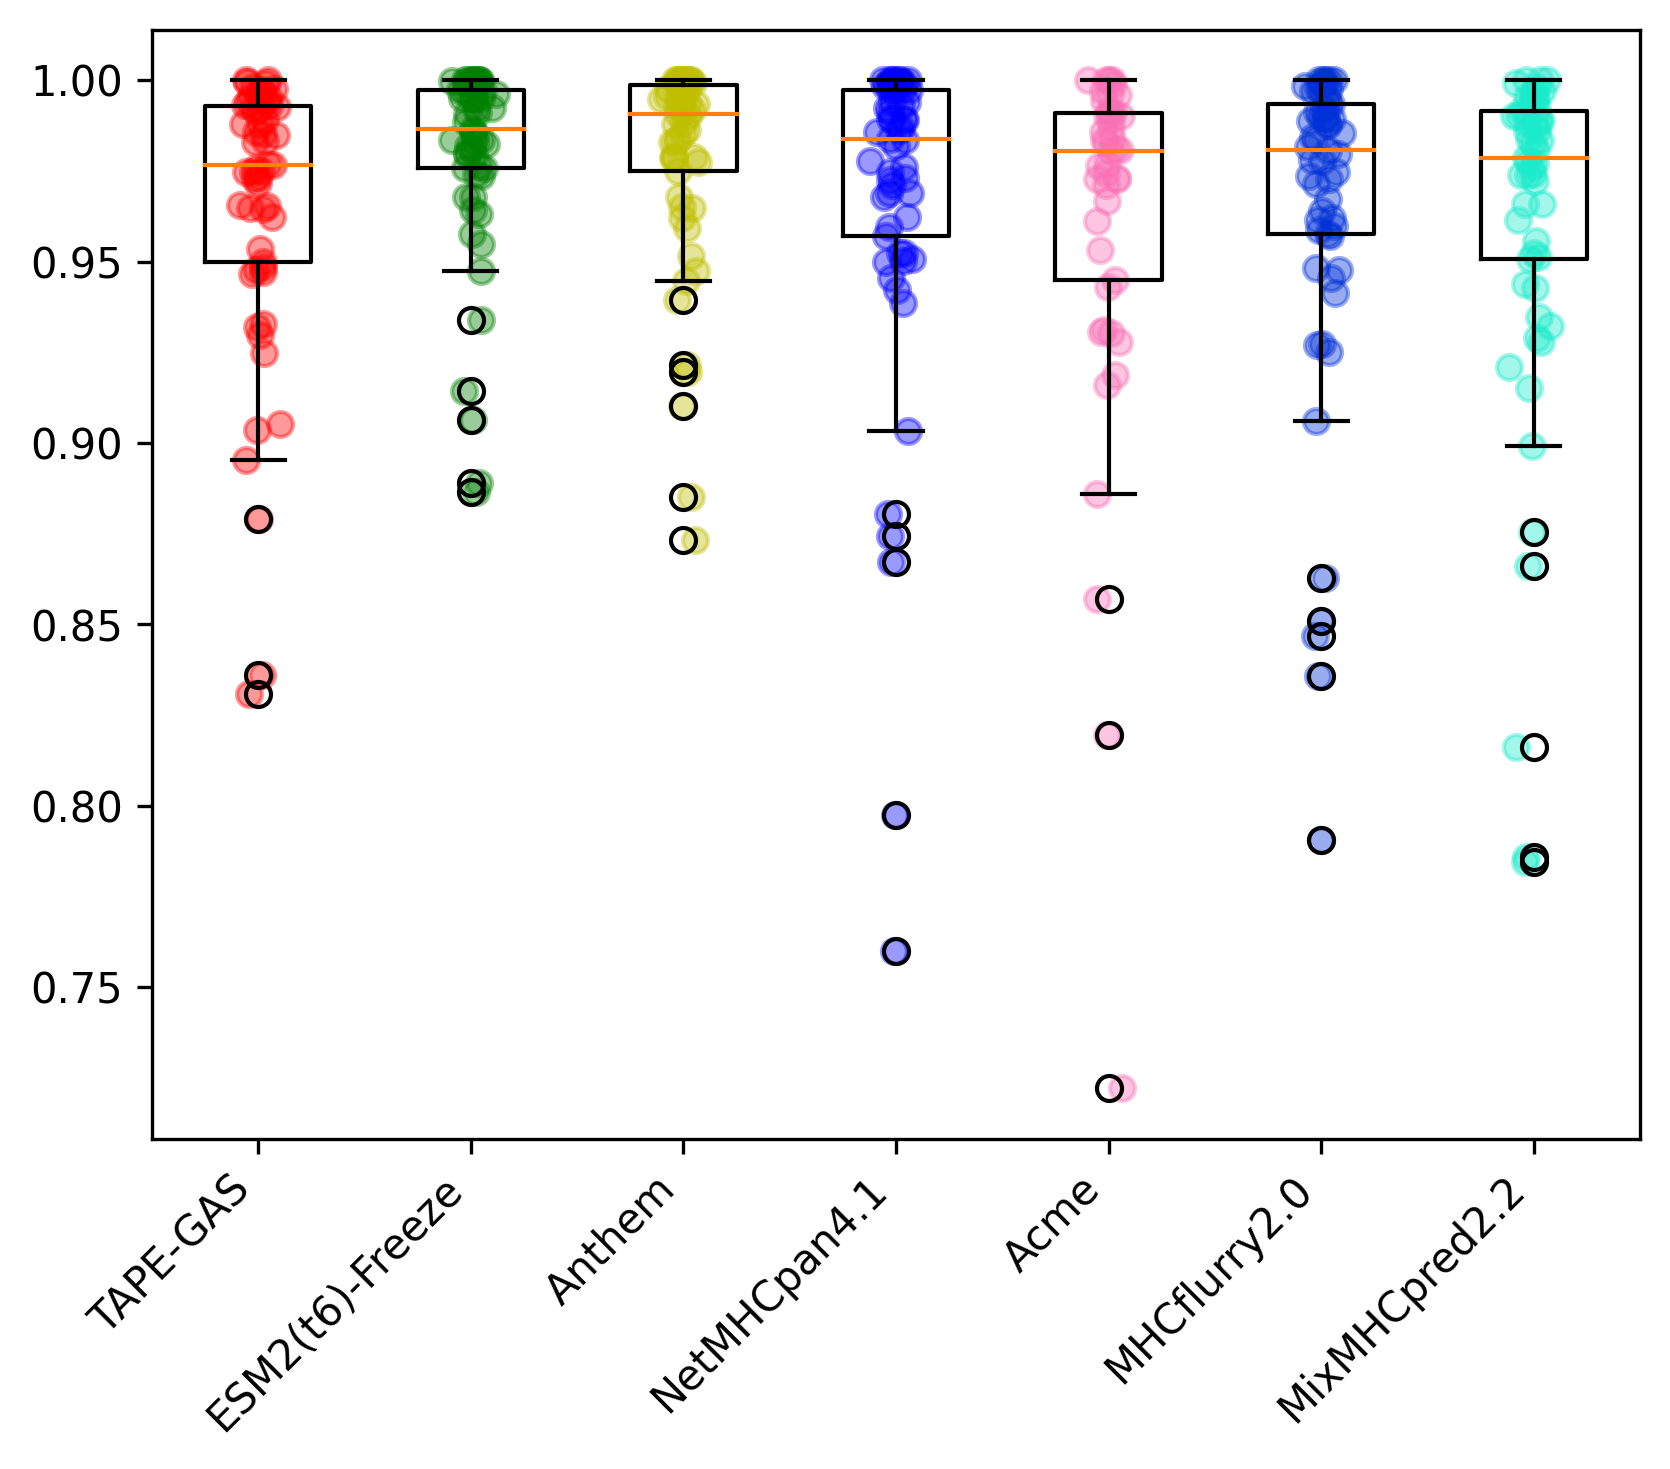
\includegraphics[width=\textwidth]{../img/results/auc_distribution_11-mer}
		\caption{11-mer}
		\label{fig:comparison_11}
	\end{subfigure}
	\hfill
	\begin{subfigure}[b]{0.3\textwidth}
		\centering
		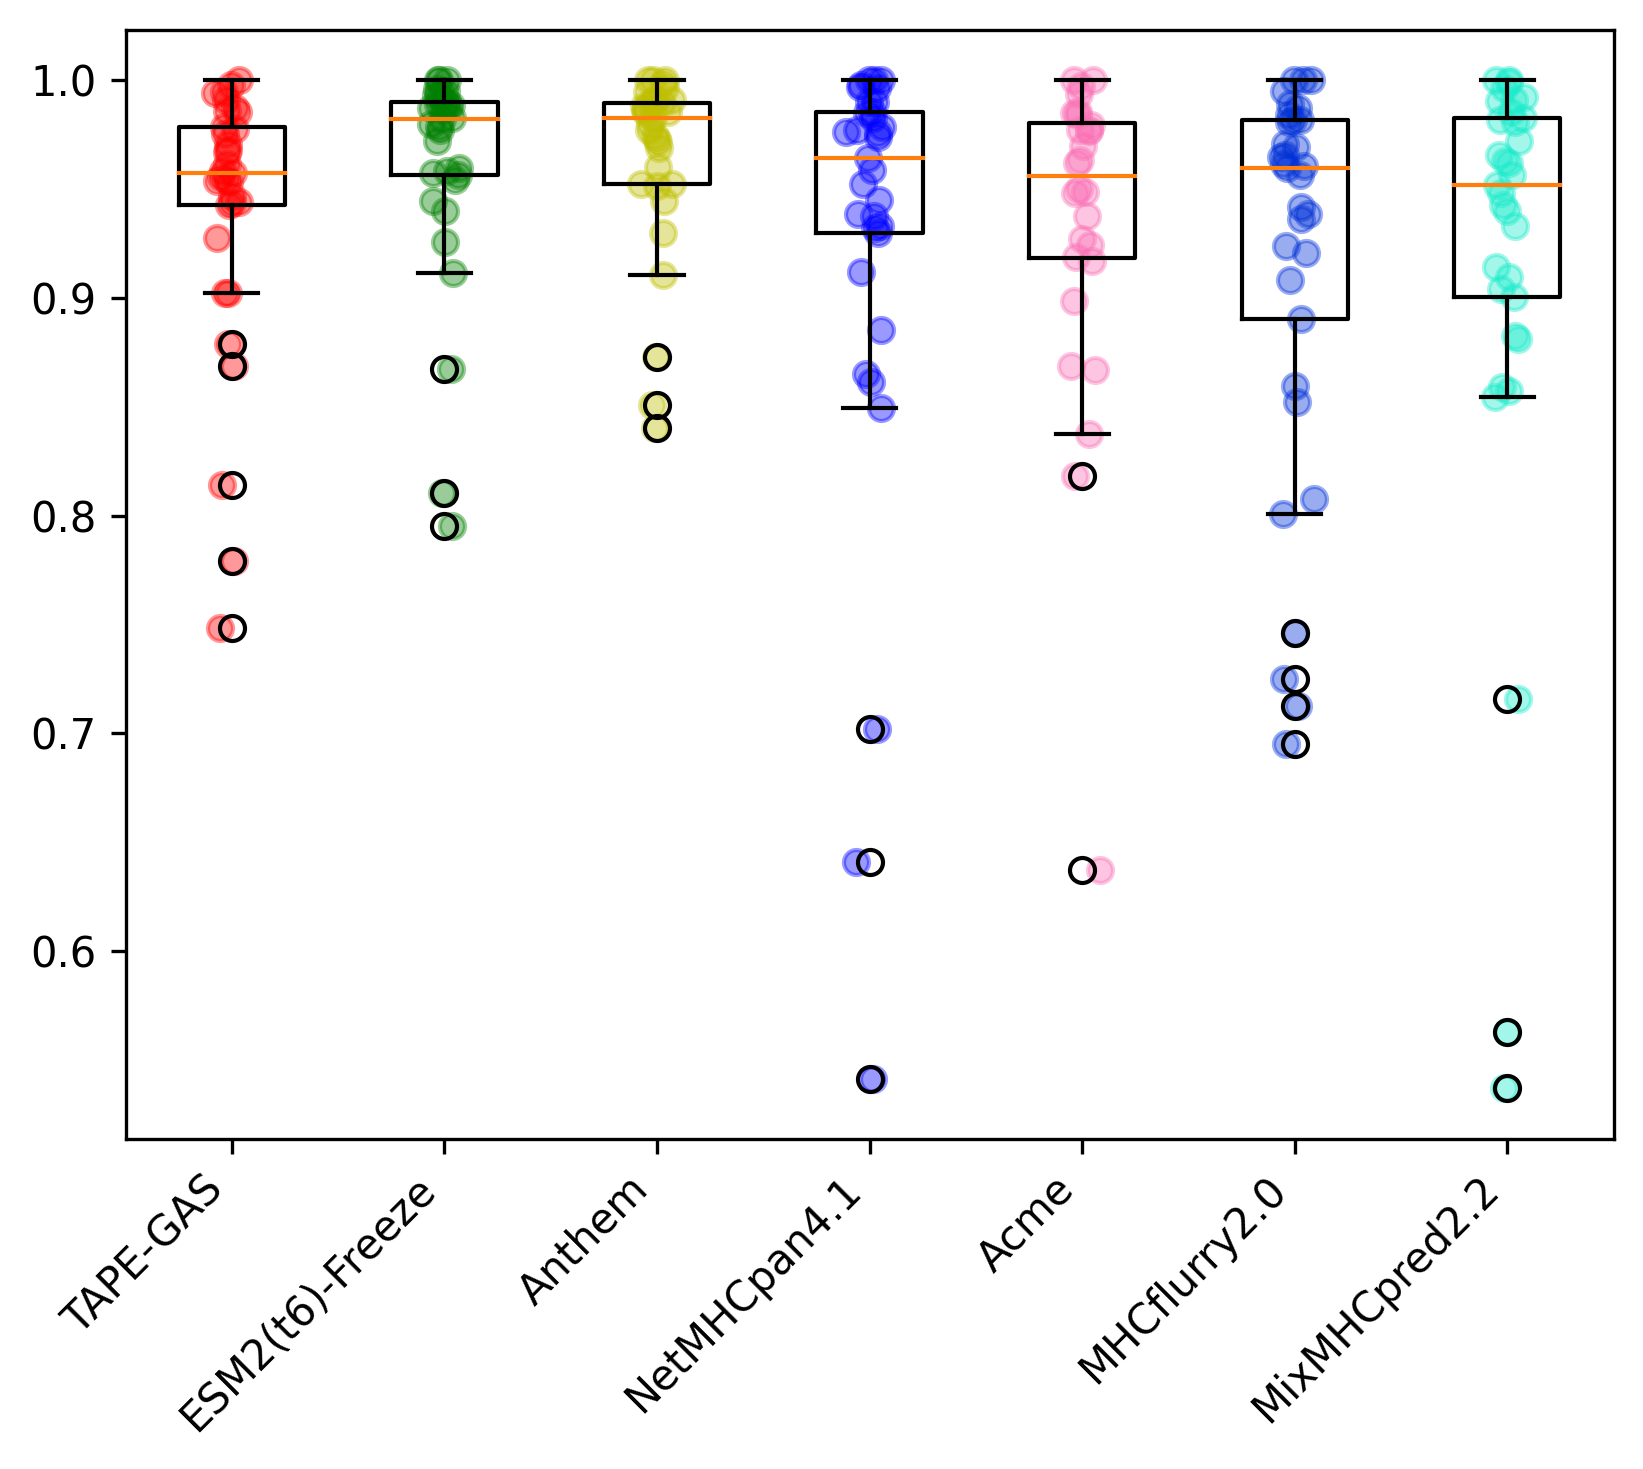
\includegraphics[width=\textwidth]{../img/results/auc_distribution_12-mer}
		\caption{12-mer}
		\label{fig:comparison_12}
	\end{subfigure}
	\hfill
	\begin{subfigure}[b]{0.3\textwidth}
		\centering
		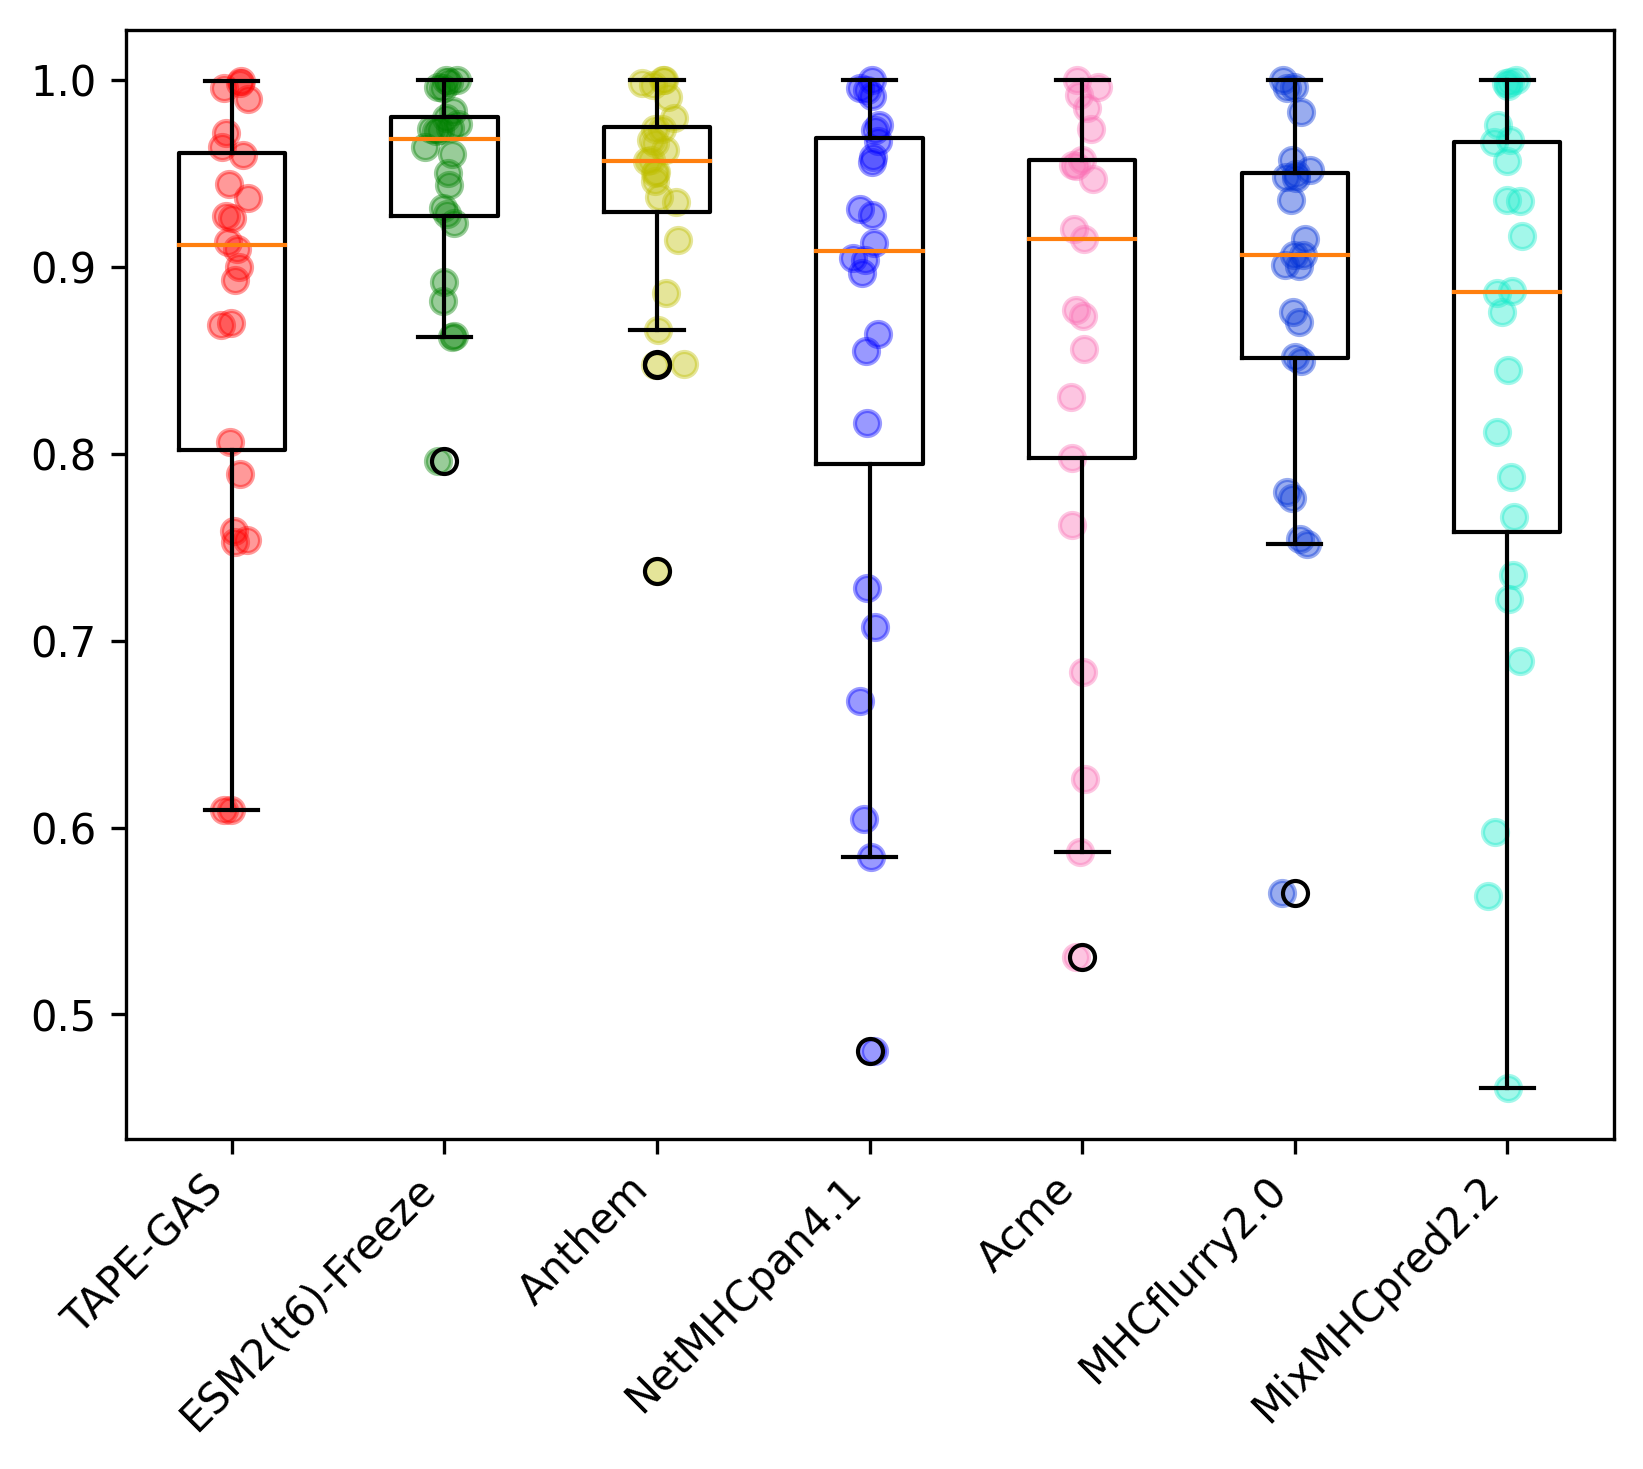
\includegraphics[width=\textwidth]{../img/results/auc_distribution_13-mer}
		\caption{13-mer}
		\label{fig:comparison_13}
	\end{subfigure}
	\hfill
	\begin{subfigure}[b]{0.3\textwidth}
		\centering
		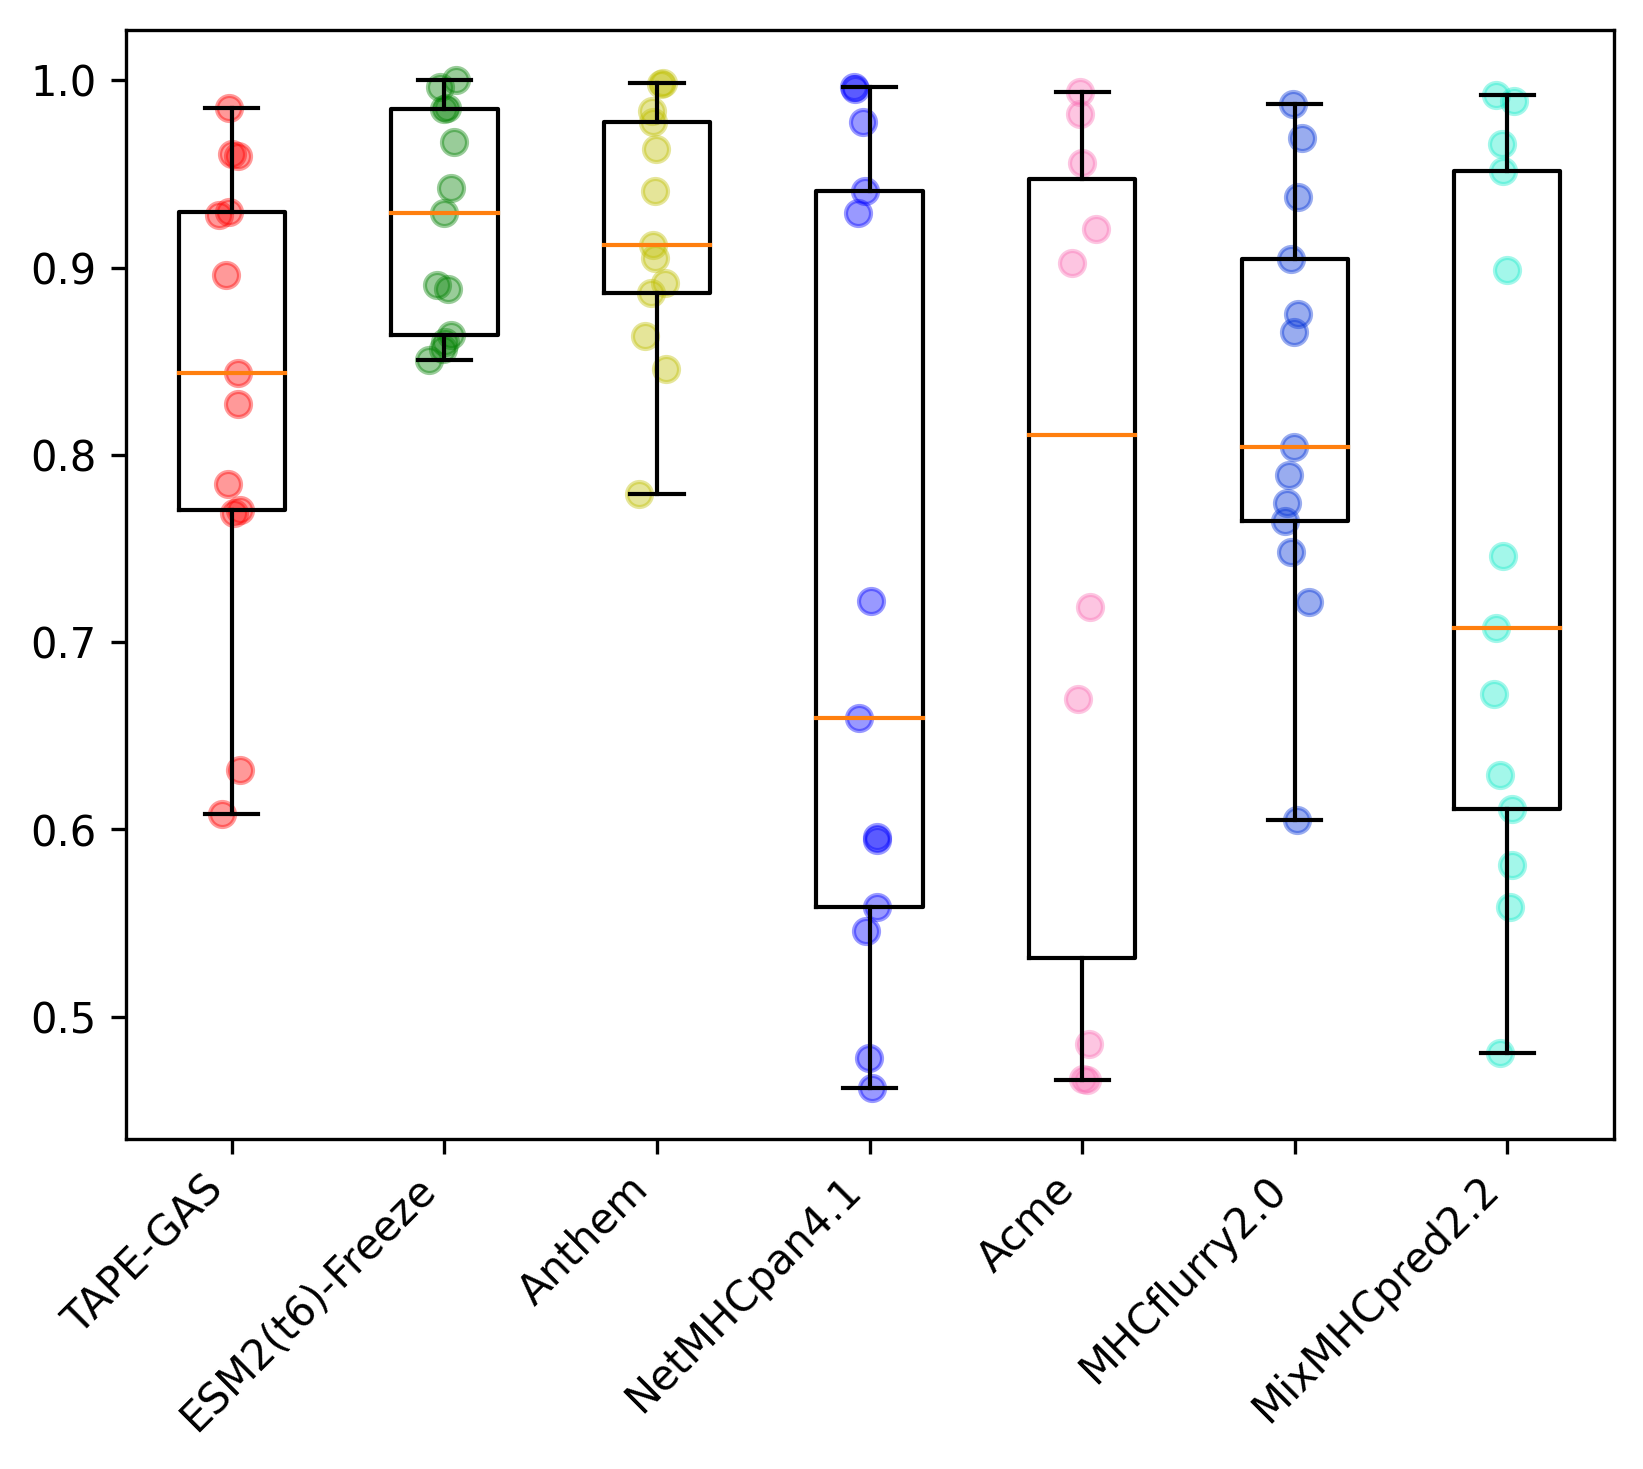
\includegraphics[width=\textwidth]{../img/results/auc_distribution_14-mer}
		\caption{14-mer}
		\label{fig:comparison_14}
	\end{subfigure}
	\caption{The AUC distribution for TAPE-GAS and ESM2(t6)-Freeze, both trained for 30 epochs, along with Anthem, NetMHCpan4.1, ACME, MixMHCpred2.2, and MHCflurry2.0.}
	\label{fig:auc_distribution}
\end{figure*}
